\chapter{Elba The Car}
The hybrid vehicle that was built upon was named Elba several years ago when it
was still a pure electric vehicle. The platform has been continuously improved
and altered to the complex hybrid that exist today. Each year Elba participates
in Shell Eco-marathon (SEM) as an ``Urban Concept Vehicle''.

%Introduction
\section{Introduction}
This section gives an introduction to Elba
\subsection{Propulsion}
Elba is an electric-ethanol hybrid vehicle which combines two 48V electrical
motors and one internal combustion engine (ICE). The electrical motors are one
0.2 kW direct current (DC) motor connected directly to the drive shaft and one
1.1 kW brushless DC motor (BLDC) connected via the clutch to the drive shaft.
The one-cylinder four-stroke ethanol powered ICE is connected to the drive
shaft via the clutch. These three provide a driving torque to the rear drive
shaft. The drive shaft is then connected to the right rear wheel via an 1:10
ratio planetary gear. The car fits a single human, he or she is also the
driver. The driver steers the car manually and decides upon a reference speed
that the car should follow and has the option to decide what motor/engine
combination that should be used at a specific time.

\subsection{Aim}
The aim of Elba is to provide a research platform to perform various levels of
projects for students from different science fields, while at the same time be
accepted to compete in SEM\@. The projects can vary in time and
extent and can be independent or made as a long term implementation.

\subsection{Shell Eco-Marathon}
SEM is a vehicle competition focused on fuel efficiency where engineering
students from around the world designs, builds and drives their own vehicles.
The competition is split into two classes. The Prototype class is solely
focused on fuel-efficiency and have less restrictions concerning comfort and
usability compared to the second class which is the UrbanConcept class,
see~\ref{UCV}.

\subsection{Urban Concept Vehicle}\label{UCV}
Elba competes in the UrbanConcept class and is what is called a UrbanConcept
Vehicle (UCV). The vehicles in this class have an appearance closer to today's
production type passenger cars. The cars in the class have to be built in
accordance with the class specific rules that dictates everything from steering
and controls to propulsion and safety. UCVs must have some common production
car features as wind shield wiper, turn signals, horn headlights etc. Vehicles
competing in this group is also required ``stop and go'' each lap, which means
that once every lap the vehicle needs to do a full stop. This is to further
increase the resemblance to city driving.

\subsection{State at start of project}
The car was in working condition when the project started, but had several
problems. To mention a few major ones: the clutch was slow and unreliable,
the overall power output might not have been enough to be efficient on the new
track, none of the potential drivers would fit in the driver compartment, the
horn disturbed the entire electrical system.

These issues where, together with the competition rules, the primary base for
the decisions that where taken and related to the car. Some of the work done to
``fix'' these problems where a matter of reshape some metal piece and bolting it
back in the car, suddenly the driver could reach the brakes. While other
required an entire team of people to get a new, working, ethanol engine in the
car.

%System Overview
\section{System Overview}
\subsection{Electronic Control Units}
The car has four electronic control units (ECUs) that are responsible for
controlling different parts of the car.

\begin{itemize}
\item Front ECU
\item Back ECU
\item ICE ECU
\item Clutch ECU
\end{itemize}

An overview of the communication between the ECUs can be seen in Figure~\ref{fig:communication_overview}

\begin{figure}[H]
    \centering\label{fig:communication_overview}
    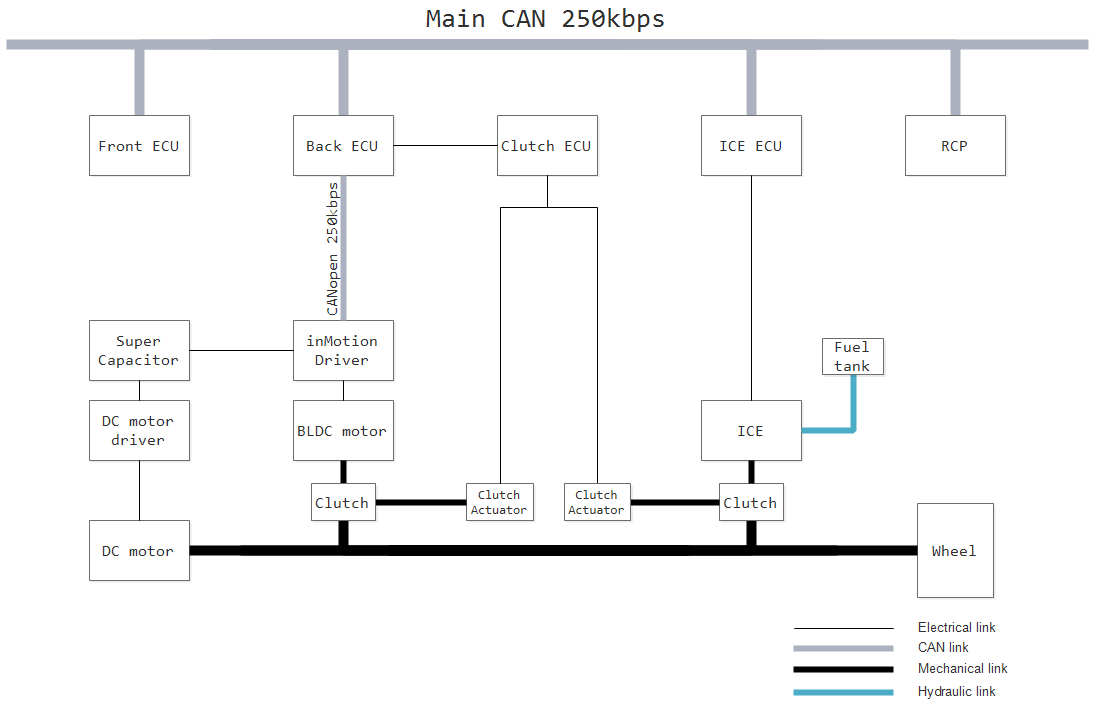
\includegraphics[width=1\textwidth]{./img/elba_communication_overview}
    \caption{Overview of the communication system and drivetrain in Elba.}
\end{figure}

The Front ECU is responsible for the human interface, the buttons where the
driver is able to decide mode and speed if the car is in manual mode. It sends
speed and drive mode on the CAN bus.

The Back ECU controls the motors via the separate motor controllers. It has
veto over the ICE and Clutch.

The internal combustion engine is controlled by the ICE ECU and this is its
only task. It senses the lambda value and motor? temperatures to control the
injection of fuel.

The Clutch ECU controls the clutch. It interfaces to two H-bridges which in turn
steers the linear actuators.  

\subsection{Communication}
The car uses a CAN network to communicate between the distributed
micro-controllers. Any data that is needed elsewhere is sent on the CAN-bus.
Each CAN message consists of a CAN id, a 32 bit upper data integer and a 32 bit
lower data integer. Messages sent from Front ECU are sent with id 170, from
Back ECU with id 169, and from ICE ECU with id 114. GPS data from the
data-logger/GPS-unit Race Capture Pro are sent with id 180. Data position in
the messages on the CAN-bus can be seen in table REF, counting the lowest bit
as bit 1. The lower data counts for bit position 1--32 and upper data 33--64.
micro-controllers. Any data that is needed elsewhere is sent on the CAN-bus. Each CAN message consists of a CAN id, a 32 bit upper data integer and a 32 bit lower data integer. Messages sent from Front ECU are sent with id 170, from Back ECU with id 169 and 113, and from ICE ECU with id 114. GPS data from the data-logger/GPS-unit Race Capture Pro are sent with id 180. Data position in the messages on the CAN-bus can be seen in table \ref{table:CAN}, counting the lowest (least significant) bit as bit 1. The lower data accounts for bit position 1-32 and upper data 33-64.

\begin{table}[H]
\label{table:CAN}
\begin{center}
\begin{tabular}{lcl}
\textbf{Data} & \textbf{Id} & \textbf{Bits}\\
\toprule
Reference Speed & 170 & 1--16 \\
Brake & 170 & 17 \\
Reference Mode & 170 & 20--23 \\
Auto & 170 & 24 \\
Current Speed & 169 & 1--16 \\
Supercapacitor Voltage & 169 & 17--32 \\ 
Current Mode & 169 & 33--36 \\ 
BLDC motor current & 169 & 37--48 \\
Distance & 169 & 49--64 \\
ICE RPM & 114 & 1--16 \\
ICE on/off & 113 & 1--2 \\
Fuel injection time & 114 & 17--32 \\
GPS longitude & 180 & 1--32 \\ 
GPS latitude & 180 & 33--64 \\
\bottomrule
\end{tabular}
\end{center}
\caption{Data position in different CAN messages on the CAN bus.}
\end{table}

Another CAN network is used between the Back-ECU and the inMotion driver that
controls the BLDC motor. This network uses the protocol CANopen that
lies on top of the CAN bus.

The instrumentation panel communicates via Bluetooth with the data-logger/GPS-unit.

\subsection{Energy supply}
All energy used to propel the car forwards (during the competition) comes from
the ethanol fuel, but electrical energy can be stored in the super-capacitor.
When the electrical motors generate energy it can be stored in this
super-capacitor for later use. The car can only start from standstill using one
of the electrical motors with energy from the super-capacitor.  

\section{Software and Simulation Models}
Using a model based approach relies on verified systems models on various
levels. Elba benefits form a full system model to simulate fuel efficiency and
each ECU has a corresponding Simulink model from which all code is compiled.

\subsection{Plant Model}
The Simulink plant model is supposed to be a full system model capable of estimating fuel consumption over an entire SEM attempt. When any component, which has an effect on propulsion, is changed on the car the plant model must also be updated. Naturally the goal with MBD is that any change can be simulated with the plant model, approved and then the car is updated. But not all simulations can be done beforehand, which was the case for the new ICE. 

Functionally, the plant model is very similar to the old one described in \cite{elba2015}. The structure of the model was improved to give a clearer view, a way of including the track profile was added and errors in some models were corrected. Also, the work of \citep{liu2016} was included in the form of a reference speed lookup table. The plant model also includes a model of the testrig to simulate forces and torques it is required to output.

Since the new ICE couldn't be properly mapped, the plant model uses parameters for the old ICE. This needs to be considered when interpreting results from simulations on the plant model.

\subsection{ECU software}
All ECUs use an Arduino (Due or Mega) as micro-controller which Simulink has
compiler support for. This means that Simulink models can be compiled and
uploaded to the Arduino directly from Simulink. The Simulink to Arduino coupling also
gives the option for running ``external mode'' a Hardware in the loop type compile mode.
This makes it possible to look at values and signals, running on the ECU, in
real-time.

\section{Data logging}
The need for collecting data a very important aspect of developing and
iterating design choices for the car in order to determine if the changes have
made the car performance and handling after the changes have been made there
is a real need for comparing data. In Elbas case there was a need for logging
data from multiple ECU's. This meant that the either the data needs to be logged
by the different ECUs themselves meaning that there might be an issue with
storage space and the data retrieving might be hazardous. The second option is
if there was the possibility to log the CAN-bus and perhaps analog and digital
channels. There was always the possibility of having the laptop in the car while
driving but this didn't seem to be the best way. After trying different things,
including making our own, the Race Capture Pro 2 (RCP2) was found to meet the
requirements, %see~\ref{app:RCP}. %%%% This gives an error %%%%%
With it's eight analogue input channels and
three digital I/O channels it is very suitable for logging both analogue and
digital signals. It also have the possibility to communicate with two
CAN-channels and logging different custom identifiers as virtual channels. This
last feature is particularly useful for the Elba project since this was one of
the requirements.

%Requirements
\section{Requirements}
\subsection{Rules}
At Shell Eco Marathon all vehicles must pass two inspections before the vehicle is allowed to enter the track. First a safety inspection evaluating if it's dangerous to have the vehicle on the track, both for the driver and other vehicles. And second a technical inspection asserting if the vehicle complies with the competition rules.

%Design Decisions
\section{Design decisions}
\subsection{Clutch decisions}
%1. What the old team told us
%2. What we told MD to do
%3. What MD did
%4. Problems still
%5. Finding the problem
%6. Fixing the arms

One of the major problems with the car has been the clutch. Figure (\ref{fig:Drivetrain}) illustrates the mechanical components of the drivetrain of elba.

\begin{figure}[H]
    \centering\label{fig:Drivetrain}
    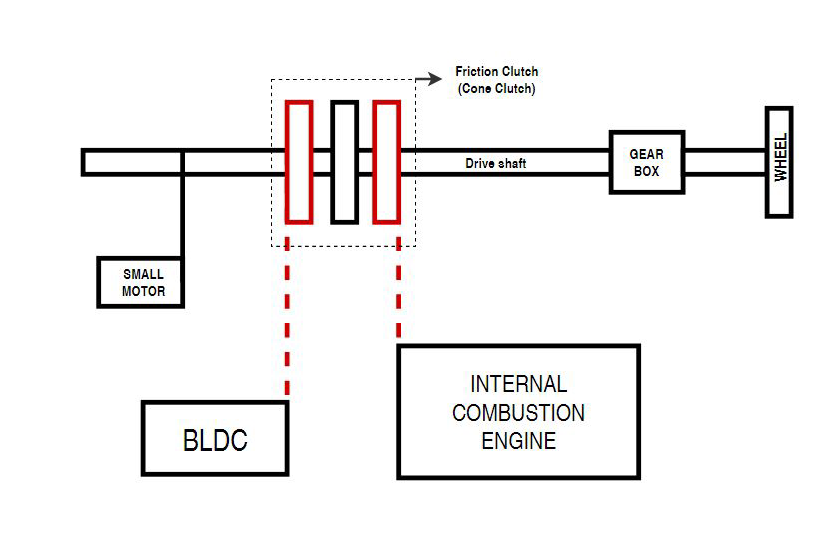
\includegraphics[width=1\textwidth]{./img/Drivetrain}
    \caption{Illustration of the mechanical components of the drive train, where the red plates can move towards the center plate to engage and disengage the motors to the drive shaft.}
\end{figure}

The Problem stated when starting the project was that the clutch actuators were oversized and thus giving more force than necessary for the clutch to engage properly. When the clutch was engaged with too much force, the clutch plate on the ICE side stuck very hard to the center plate and could not be disengaged using the actuator.

To solve the mechanical problems it was decided to appoint one team from the machine design department to work solely on the mechanical parts of the clutch. The mechatronics team decided to completely remake the clutch ECU to make it more robust. Despite the new ECU and the work performed by the machine design team, which can be read about in (TODO REPORT.XX) there was problems with the clutch when it was time to race. The problems was of the same mechanical nature as before the rework, where the clutch plate on the ICE side could not be disengaged from the drivetrain.

To solve this problem, several solutions have been investigated. The clutch mechanism has been controlled by time rather than position. One approach was to use the built in hall sensor in the actuator to control the position. One other idea was to use an external current sensor on the clutch ECU to control the position. A third idea was to continue using time as reference, but increase it so that an end position is always reached, which can be used as a reference position.

When investigating alternative three above using longer time to engage and disengage the clutch a new problem was discovered. It appeared that even though the clutch was not stuck to the center plate it still could not be properly disengaged. This was due to the geometry of the lever arm which pushes the clutch plate.  After this important insight the drivetrain was disassembled and new lever arms were constructed and manufactured. When the drivetrain was assembled again the clutch worked like a charm. Figure (\ref{fig:clutch}) is a rendered image of one of the new lever arms.

%%TODO
\begin{figure}[H]
    \centering\label{fig:clutch}
    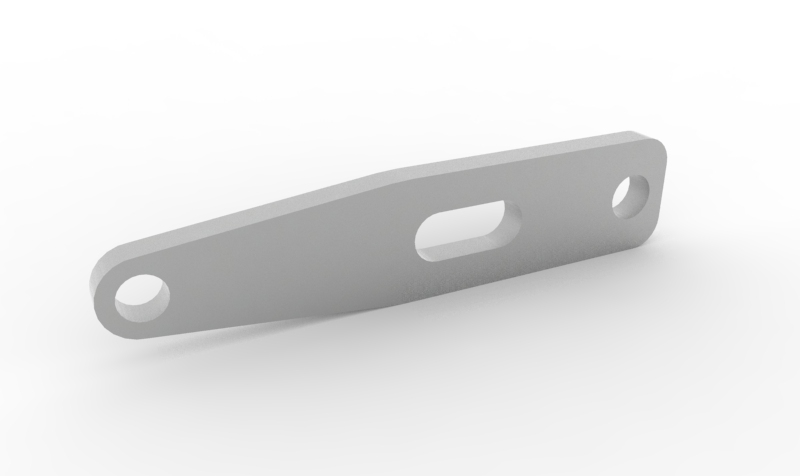
\includegraphics[width=1\textwidth]{./img/clutch}
    \caption{The new clutch lever arms}
\end{figure}

\subsection{Internal Combustion Engine and ICE ECU}
It was decided that this years car should compete in the alternative fuels
class. This means that the car should be powered by an engine that runs on
ethanol. An engine running on ethanol needs to have a higher compression ratio than
a petrol engine.
%% TODO: Source on the above. Also, link to ICE report.
The requirements engineering and modifications on the new ICE was set by the ICE
team. To control the new engine, a new ICE ECU was needed. It was also decided
that the new ICE ECU would contain more sensor inputs as well as the possibility
to control the ICE ignition. All functionality of the old ICE ECU would still be
present, namely:
\begin{itemize}
    \item Simulink TLC software.
    \item Feedback control loop of injection time.
    \item Lambda value sensing.
    \item Encoder reading with index pulse from ICE\@.
\end{itemize}
More sensor data together with ignition control would give possibilities
for more exact control of the ICE\@. The extra features of the new ECU were:
\begin{itemize}
    \item Motor oil temperature sensing.
    \item Ambient air temperature sensing.
    \item Ignition control.
\end{itemize}
The features were implemented on the ECU PCB and the system was designed so that
the sensors and features could be implemented incrementally according to the
time and need of the project. Given that the amount of time that would be needed
to get the car in working condition before the race was not easily planned
beforehand, it was beneficial to have a base functionality with flexibility to
add features.

\subsection{Door}
The car is required to have a door, with a large enough entrance and working
locking mechanism \cite{semrules16c1}. Since the old, layered carbon fibre door
was too flimsy and also back hinged (there is a reason its called ``suicide door''),
it was decided a new, sturdier, door would be made. Two lightweight-construction
student took this upon them self as a bachelors project. 

The new door where constructed in a carbon fibre sandwich style and was open in
a scissor manner. The door became sturdier but the hinges where less than ideal
and the closing mechanism did not work.

%Results
\section{Results}
We beat Chalmers. We are no byskola.

\subsection{Competition}
At the time the team arrived in London the ICE had never been started with only ethanol as fuel, the door had to be mounted and the team needed to do a number of small changes to be able to pass both inspections. Most time was spent to get the engine running, but it was never able to run for more than a couple of strokes. 

Both the technical inspection and safety inspection were passed. There where a few complaints: The doors closing mechanism where insufficient, the indicator lights where to weak, and the fire-extinguishers expirations data had passed. All these had to be reinspected before Elba was given a pass.

It was decided that one attempt should be made even if the engine never had been started properly. Since the car must be rolling to start the ICE the inertia of the car will keep the ICE turning even if it misfires (the wheel inertia is not enough for this). This meant that the ICE started once the car finally was running during the attempt. %But it was soon discovered that the engine could not be shut off, if the clutch was disengaged the engine kept running and revving at dangerous levels. %KOMMENTAR: Känns som att vi kan utelämna denna bit... :D /Emil
At the compulsory stop after one lap the clutch to the ICE did not properly disengage, causing Elba to stall the engine with clutch engaged. While trying to get going again the clutch could not be disengaged and the attempt had to be aborted.

Therefore Elba never got a competition result. But many lessons where learned.

\subsection{End of project}

\section{Conclusion}
